%!TEX root = ../../report.tex
\section{Mapping with Location noise}

\subsection{Monte Carlo localization}

AMCL

Scan map with location noise and AMCL
Considerations on noise. What types of noise are present. Estimation of the noise. Comparison between estimation and actual error (of bags) 
Non-ideal Inverse Sensor Model
From hector

\subsection{Monte Carlo Integration Inverse Sensor Model}

\cite{monteCarloIntegration}

\subsection{Cone based model}
An attempt to represent the pose uncertainty in the static mapping is model based on a sonar-like cone. The idea is to represent the uncertainty of origin position and angle of each laser ray with a broad centered cone. 
This cone, which can be seen in figure  \ref{fig:cone_with_noise_top}, consist of three areas. These are the center, the left side cone and right side cone. As the model is based on a sonar cone model [REFERENCE TO SONARCONE], the values of a cell is determined by the distance from the origin and the angle to the straight line to the target. The changes from the original sonar model is the center section which splits the two cone halves. 

The angle \(\theta\) is equal to the standard deviation of the orientation estimate. 
The width of the center area, w, is determined by the sum of the projection of the standard deviation in the x and y directions perpendicular to the ray direction. 

The value of a cell is determined by the distance from the origin line. [For instance the value at the point p in figure \ref{fig:cone_with_noise_top} is determined by the the distance l.] The width, m, of the marking cone is determined by the position error projected onto the ray.




\begin{figure}
	\centering
			\includegraphics[width=\textwidth]{figures/static_mapping/cone_noise_top}
			\caption{Cone representing pose noise}
			\label{fig:cone_with_noise_top}

\end{figure}

Simulation of Mapping with Location Noise
Comparison
Efficiency - Computational price\\ 
 \\

In order to compare the various mapping methods a metric for determining the accuracy of a map. One of the methods for comparing to occupancy maps is the MapScore, first proposed in [REFERENCE TO ELFES MAPSCORE]. The score is calculated as the squared error between the occupancy for each cell in two maps, as seen in equation \ref{eq:MapScore}.

\begin{equation}
\label{eq:MapScore}
Score = \sum_{n=0}^{N} (m_{n} - o_{n})^2
\end{equation}

N is all cells in the maps m and o. This gives a simple result that indicates how alike two maps are. However, as most maps contains vastly more free space than occupied space this might skew the result. A map can receive a higher score for asserting strong statements about free cells but not mapping obstacles very accurate. As the obstacles are a vital part of the map this is not desired. To overcome this it is suggested to only use cells where either one of the maps have an occupied probability higher than \(0.5\) [REFERENCE TO EVAL OF MAP METHODOLEGIES]. If the MapScore is to be used to evaluate a mapping algorithm between different maps, it is necessary to normalize the score with the number of cells in the map tested. 

\begin{figure}
	\centering
	\includegraphics[width=0.7\linewidth]{figures/static_mapping/particle_sensor}
	\caption{Example map with few scans from the five highest weighted particles.}
	\label{fig:particle_sensor}
\end{figure}

\begin{figure}
	\centering
	\begin{subfigure}[b]{0.45\textwidth}
		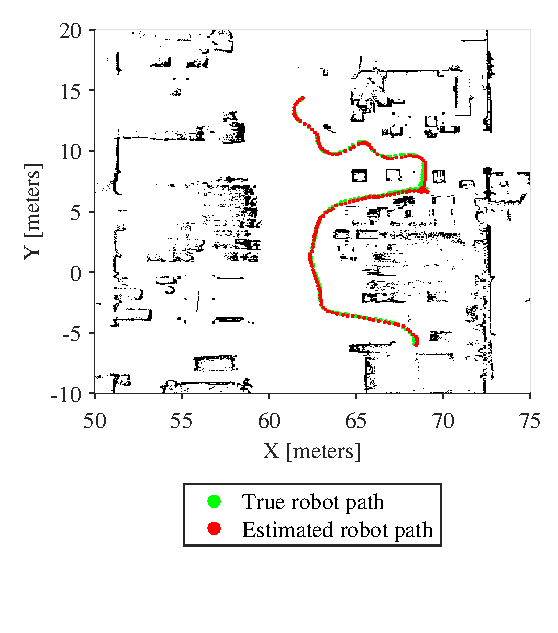
\includegraphics[width=\textwidth]{figures/static_mapping/map_with_poses}
		\caption{World represenation}
		\label{fig:simulated_robot_estimate_total}
	\end{subfigure}
	~ %add desired spacing between images, e. g. ~, \quad, \qquad, \hfill etc. 
	%(or a blank line to force the subfigure onto a new line)
	\begin{subfigure}[b]{0.45\textwidth}
		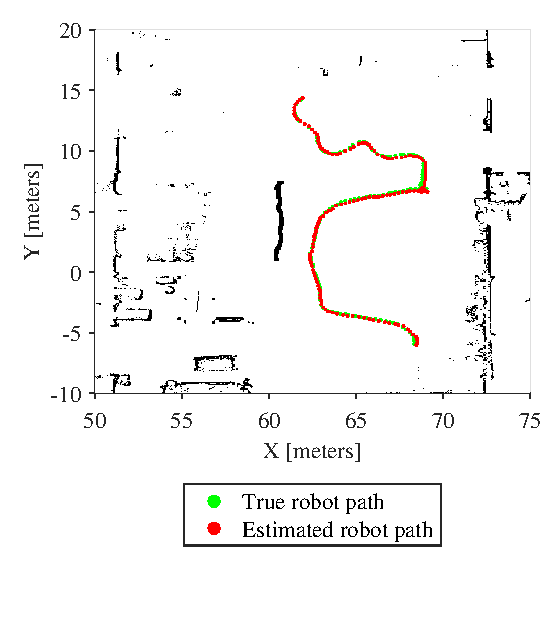
\includegraphics[width=\textwidth]{figures/static_mapping/amcl_map_with_poses}
		\caption{Map used by AMCL}
		\label{fig:simulated_robot_estimate_total_edited}
	\end{subfigure}
	\caption{Simulation of a MIR robot moving with imprecise location.}
	\label{fig:animals}
\end{figure}

